\documentclass[a4paper,10pt,twoside]{article}
\usepackage[utf8]{inputenc}
\usepackage[french]{babel}
\usepackage[T1]{fontenc}
\usepackage{amsmath}
\usepackage{amsfonts}
\usepackage{amssymb}
\usepackage{graphicx}
\usepackage{multicol}
\usepackage{array}
\usepackage{float}
\usepackage{epstopdf}
\usepackage[justification=centering]{caption}
\usepackage{caption}
\usepackage{subfig}
\usepackage{gensymb}
\usepackage[bottom]{footmisc}
\usepackage{appendix}
\usepackage{pdfpages}
\usepackage{todonotes}
\usepackage{mathpazo}
\usepackage{titleps}
\usepackage{color}
\usepackage{hyperref}
\usepackage[skins]{tcolorbox}
\usepackage{sectsty}
\usepackage[arrowmos]{circuitikz}
\usepackage{blindtext}
\usepackage{adjustbox}
\usepackage{listings}
\usepackage[inner=2.5cm,outer=2.5cm,top=3cm,bottom=3cm]{geometry}

\graphicspath{{pictures/}}
\setlength\parindent{0pt}
\renewcommand*\rmdefault{ppl}
\newcolumntype{C}[1]{>{\centering\let\newline\\\arraybackslash\hspace{0pt}}m{#1}}
\newcolumntype{R}[1]{>{\raggedright\arraybackslash}p{#1}}
\sectionfont{\large}
\subsectionfont{\normalsize}

% Page style definitions
\newpagestyle{main}{
	\sethead[Club ELEC : Hands-on 3][][]  % even
			{\chaptertitle}{}{Club ELEC : Hands-on 3}
	\headrule
    \setfoot[\thepage][][]
    		{}{}{\thepage}
}

\newpagestyle{appendix}{
	\sethead[Club ELEC : Annexes][][]  % even
			{}{}{Club ELEC : Annexes}
	\headrule
    \setfoot[\thepage][][]
    		{}{}{\thepage}
    \footrule
}

%----------------------------------------------------------------------------------------
%	TITLE SECTION
%----------------------------------------------------------------------------------------
\title{
	\vspace{2.5cm}
	\normalfont \normalsize
	\huge Club ELEC\\
	\vspace{2.5cm}
	\huge Projet Robot\\
	\vspace{.25cm}
	\Large HO3 - Détection de ligne
	\vspace{2.5cm}
	\centering
}

\begin{document}
\renewcommand{\figurename}{Fig.}
\renewcommand{\thepage}{\roman{page}}
\setcounter{page}{1}

\pagenumbering{gobble}
\maketitle
\newpage
\pagenumbering{arabic}
\pagestyle{main}

\newpage
\null
\thispagestyle{empty}
\newpage
\clearpage

\setcounter{page}{1}

%%% Introduction
\section*{Introduction}
Pendant ce quadrimestre, le Club ELEC vous propose de développer un petit robot contrôlé par une télécommande à infrarouges. Pour ce faire, le développement du circuit se déroulera en 3 phases, chacune correspondant à une séance de hands-on proposée par le club.

\begin{itemize}
	\item[-] HO1: Contrôle des moteurs.
	\item[-] HO2: Télécommande infrarouges et programmation.
	\item[-] HO3: Assemblage du robot.
\end{itemize}

%%% Objectifs du HO1
\section*{Objectifs}
Les objectifs du premier hands-on sont:
\begin{itemize}
	\item[-] De se familiariser avec le matérial de base (breadboard, multimètre, oscilloscope) et les composants de base (résistances, capacités, amplificateurs opérationnels, composants intégrés) propres à l'électronique.
	\item[-] De comprendre le fonctionnement du circuit de contrôle du moteur, basé sur des signaux de contrôle adéquats et d'un pont H.
	\item[-] De connecter ce circuit à un moteur DC pour en vérifier le bon fonctionnement.
\end{itemize}

%%% Assemblage du robot
\section*{Connexion des blocs}
Pour la connexion des différentes parties découvertes lors des dernières séances, vous devriez être maintenant capables de vous en sortir avec les informations déjà reçues. Si vous avez la moindre question, les membres du Club se feront un plaisir de vous aider!\\

Jusqu'ici, vos circuits étaient alimentés par une tension de 5V, provenant soit d'une source fixe ou soit d'un câble USB. Pour rendre votre robot autonome dans ses déplacements, vous recevrez une pile 9V ainsi qu'un connecteur. Connectez les masses ensemble et la tension positive de la pile (fil rouge du connecteur) au port VIN de l'Arduino. Ce port permet de recevoir une tension d'alimentation entre 7V et 12V, qui est réduite à 5V par un régulateur interne de l'Arduino. Cette tension de 5V est utilisée par l'Arduino pour fonctionner et peut également être utilisée pour alimenter des circuits externes (par exemple le récepteur infrarouge) grâce à la sortie 5V. Comme le moteur consomme beaucoup de puissance, pour éviter de surcharger le régulateur de tension de l'Arduino, ne branchez pas l'alimentation $V_{DD,moteur}$ (cfr. hands-on 1) sur le 5V mais directement sur le 9V de la pile. Cela permettra également au moteur de tourner plus vite. ATTENTION! Ne branchez pas le 9V sur $V_{DD,controle}$, qui reste branché sur le 5V.\\



\section*{Assemblage du robot}
Pour l'assemblage du robot, vous êtes libres d'utiliser la structure que vous préférez, laissez libre cours à votre imagination! Nous aurons préparé un peu de matériel dont vous pouvez vous servir, mais libre à vous d'en utiliser d'autres. Pour participer au concours qui aura lieu dans quelques semaines, référez vous au règlement pour connaitre les quelques contraintes pour la structure finale de votre robot.

%%% Détection de ligne
\section*{Détection de ligne}
Une partie du concours sera réservée aux robots capables de suivre une ligne tracée au sol, indépendamment de tout contrôle humain. Si vous désirez y participer, vous trouverez ci-dessous les instructions pour la connexion du capteur et la programmation de l'Arduino. \\

Comme illustré à la Figure~\ref{fig:circuit}, la détection d'une ligne se fait à partir d'une LED et d'une photodiode. Le principe de base du fonctionnement est assez simple: la LED éclaire une surface et la photodiode mesure la partie de la lumière qui est réfléchie. En fonction de la couleur de la surface, plus ou moins de lumière sera réfléchie, ce qui permet donc de déterminer si on est au-dessus d'une ligne noire ou au-dessus d'une surface blache à partir de la mesure de la photodiode.\\

La façon dont le circuit de lecture de la photodiode fonctionne est un peu plus subtile. Les plus attentifs auront peut-être remarqué que la diode semble être branchée à l'envers, dans le sens non-passant avec la cathode du côté positif et l'anode du côté négatif. Du coup, comment fait-on pour effectuer une mesure si aucun courant ne passe? En réalité, quand une diode est branchée dans le sens non-passant, un courant très faible passe néanmoins. Dans une photodiode, ce courant va dépendre de la quantité de lumière reçue dans un certain intervalle de longueurs d'ondes (dans notre cas pour des lumières infrarouges). Ce courant qui varie, de l'ordre de quelques nA dans le noir à plusieurs $\mu$A à la lumière, passe à travers une résistance, ce qui crée donc une variation de la différence de potentiel. En lisant la tension grâce à l'ADC de l'Arduino sur la broche A0, on peut donc détecter un changement de lumière.\\

\begin{figure}[!t]
\centering
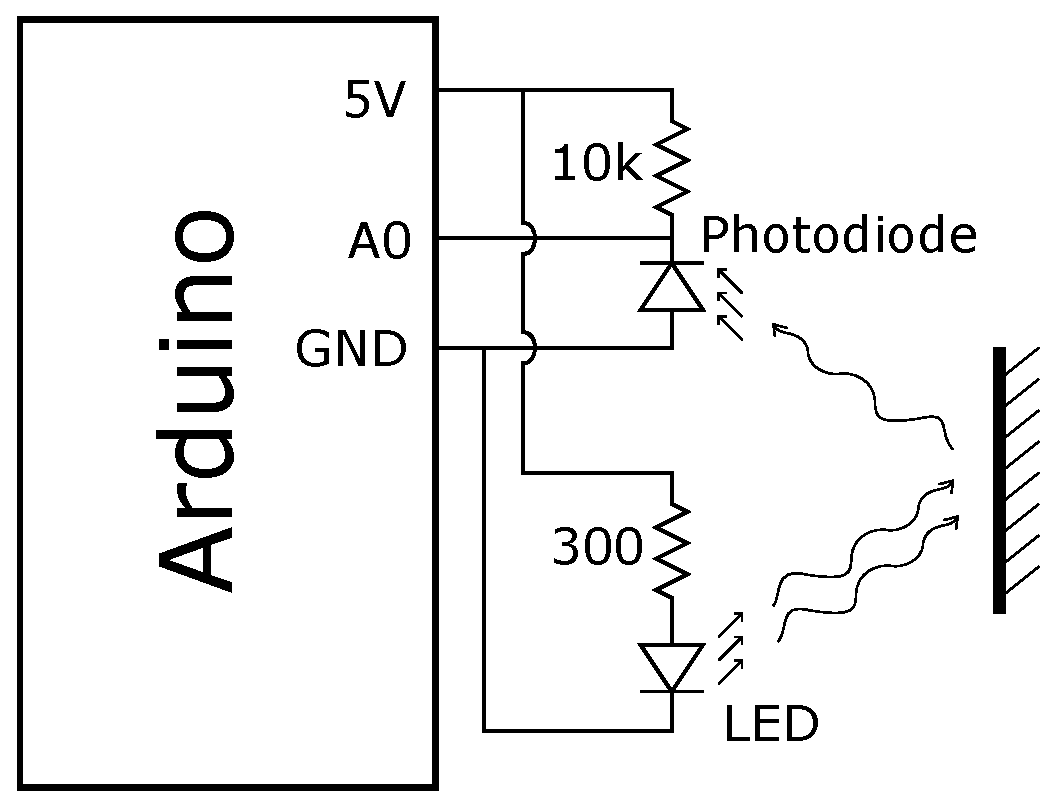
\includegraphics[width=0.4\textwidth]{imgs/circuit.eps}
\caption{Circuit et principe de fonctionnement pour la détection de ligne.}
\label{fig:circuit}
\end{figure}

Dans le code, la lecture de la tension se fait grâce à la fonction \textit{analogRead(pin)}. Vous pouvez faire l'essai avec le morceau de code ci-dessous. Observez le changement de ce qui s'affiche dans le terminal en fonction de la surface qui fait face au capteur. 

\lstset{language=C}
\begin{lstlisting}[frame=single,numbers=left,numberstyle=\small,label={code1},caption={Lecture de la photodiode.}]
const int PHOTO_PIN = 14;

int val = 0; 

void setup() {
  Serial.begin(9600); 
}

void loop() {
  val = analogRead(analogPin);  
  Serial.println(val);      
  delay(300);
}

\end{lstlisting}

A partir de cette valeur, vous pouvez maintenant essayer de programmer le contrôle du mouvement de votre robot. Il existe énormément de stratégies possibles, des très simples aux plus compliquées, avec un ou plusieurs capteurs. A vous de réfléchir à ce que votre robot doit viser comme valeur sur les capteurs, quand et comment tourner pour rester le plus proche possible de la ligne... Pour vous aider, n'hésitez pas à aller faire un tour sur Internet, certains projets en ligne pourront probablement vous aider!

\end{document}
